\documentclass[a4paper]{article}

\usepackage{Sweave} %--------------------------------!
\usepackage{amsmath}
\usepackage{amssymb}
\usepackage{amsthm}
\usepackage{fancyhdr}
\usepackage[usenames, dvipsnames]{color}
\usepackage{verbatim}

\oddsidemargin 0cm
\topmargin -2.4cm     %I recommend adding these three lines to increase the
\textwidth 16.5cm   %amount of usable space on the page (and save trees)
\textheight 27.5cm

\newcommand{\question}[2] {\vspace{.25in} \hrule\vspace{0.5em}
\noindent{\bf #1: #2} \vspace{0.5em}
\hrule \vspace{.10in}}
\renewcommand{\part}[1] {\vspace{.10in} {\bf (#1)}}

\newcommand{\myname}{Xuan Han}
\newcommand{\myhusky}{han.xua@husky.neu}
\newcommand{\myhwnum}{5}

\setlength{\parindent}{0pt}
\setlength{\parskip}{5pt plus 1pt}

\pagestyle{fancyplain}
\lhead{\fancyplain{}{\textbf{HW\myhwnum}}}      % Note the different brackets!
\rhead{\fancyplain{}{\myname\\ \myhusky}}
\chead{\fancyplain{}{8 9 9}}


\begin{document}
\Sconcordance{concordance:crossvalidation.tex:crossvalidation.Rnw:%
1 46 1 1 2 1 0 3 1 3 0 1 2 8 1 1 2 5 0 1 2 7 1 1 2 1 0 4 1 1 4 3 0 1 1 %
6 0 1 2 2 1 1 2 1 0 1 1 1 4 3 0 1 1 6 0 1 2 17 1 1 2 1 0 1 1 7 0 2 1 8 %
0 2 1 9 0 2 1 14 0 1 3 8 1 1 2 1 0 1 2 1 0 5 1 6 0 1 2 1 1 1 2 1 0 1 1 %
6 0 1 2 6 1 1 2 1 0 1 1 15 0 1 2 6 1 1 2 1 0 2 1 5 0 1 1 15 0 1 2 6 1 1 %
2 1 0 1 1 6 0 1 2 1 1 1 2 1 0 1 1 15 0 1 2 7 1 1 2 8 0 1 2 1 1 1 2 1 0 %
1 1 15 0 1 2 10 1 1 2 1 0 4 1 3 0 1 2 1 1 1 2 1 0 2 1 6 0 1 2 1 1 1 2 1 %
0 8 1 5 0 5 1 7 0 1 2 1 1 1 2 1 0 4 1 5 0 3 1 5 0 2 1 17 0 1 2 9 1 1 2 %
1 0 4 1 5 0 1 1 5 0 1 1 6 0 1 2 5 1}


\title{Data Mining Assignment \myhwnum}
\author{\myname \\
        \myhusky}
\date{\today}
\maketitle

\thispagestyle{plain}


\question{8}{Cross validation}
\part{a}
\begin{Schunk}
\begin{Sinput}
> set.seed(1)
> y = rnorm(100)
> x = rnorm(100)
> y = x - 2 * x^2 + rnorm(100)
\end{Sinput}
\end{Schunk}
{\color{red}
\begin{enumerate}
\item In this data set, n = 100, p = 2
\item $Y$ = $X - 2X^2 + \epsilon$
\end{enumerate}
}


\part{b}
\begin{Schunk}
\begin{Sinput}
> plot(y ~ x, col = 'blue')
\end{Sinput}
\end{Schunk}
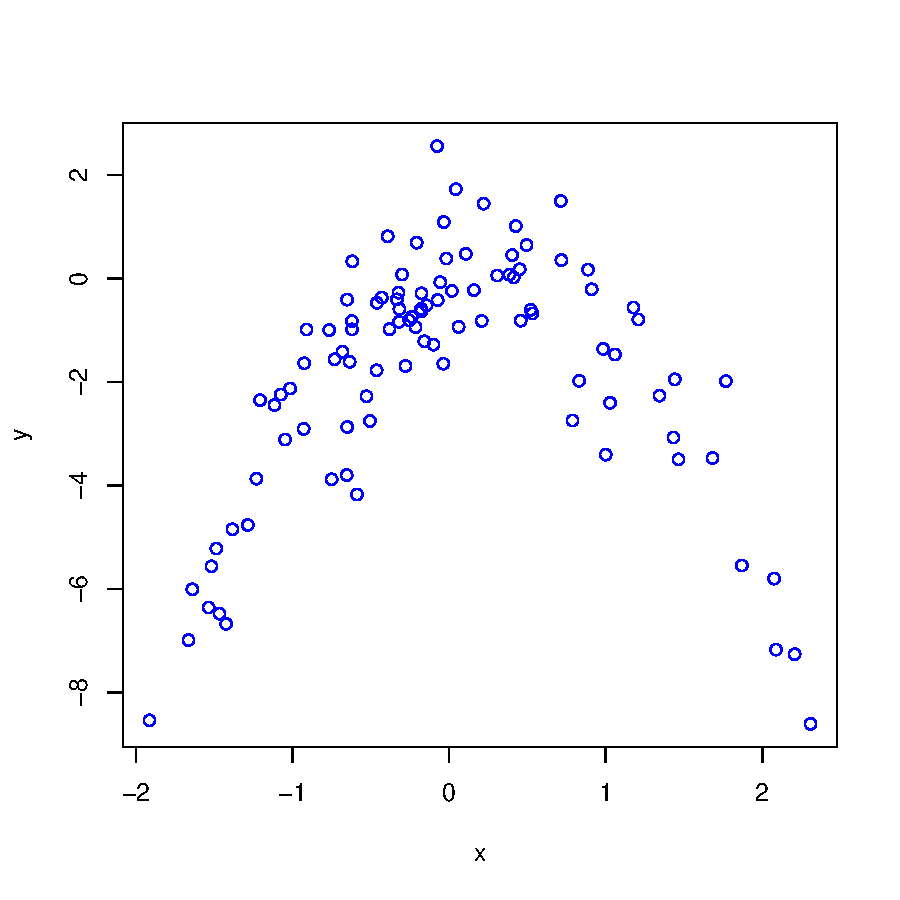
\includegraphics{crossvalidation-8b}
{\color{red}
\begin{enumerate}
\item We can see that the data points are distributed along a parabola, just as we expected.
\item x goes from -2 to 2, y goes from -8 to 2.
\end{enumerate}
}

\part{c}
\begin{Schunk}
\begin{Sinput}
> library(boot)
> set.seed(12)
> df = data.frame(X = x, Y = y)
> p = 4
> loocv.err = rep(NA, p)
> for(i in 1:p) {
+     glm.fit = glm(Y ~ poly(X, i), data = df)
+     loocv.err[i] = cv.glm(df, glm.fit)$delta[1]
+ }
> loocv.err
\end{Sinput}
\begin{Soutput}
[1] 5.890979 1.086596 1.102585 1.114772
\end{Soutput}
\end{Schunk}


\part{d}
\begin{Schunk}
\begin{Sinput}
> set.seed(2015)
> loocv.err = rep(NA, p)
> for(i in 1:p) {
+     glm.fit = glm(Y ~ poly(X, i), data = df)
+     loocv.err[i] = cv.glm(df, glm.fit)$delta[1]
+ }
> loocv.err
\end{Sinput}
\begin{Soutput}
[1] 5.890979 1.086596 1.102585 1.114772
\end{Soutput}
\end{Schunk}
{\color{red}
\begin{enumerate}
\item The results obtained are exactly the same.
\item The reason is that for leave-one-out-CV, the results have nonthing to do with seed. It will evaluate 100 times no matter what the seed is. There is no randomness involved in the process of LOOCV.
\end{enumerate}
}


\part{e}
{\color{red}
\begin{enumerate}
\item The second model have the smallest LSSCV error. This is exactly what I expected.
\item Because the simulated data set is generated by power of 2 of X, if we use a lower order model such as power of 1 of X, it will have high bias; If we use a higher order model such as power of 3 or 4 of X, it will cause high variance. So, power of 2 have low bias and low variance.
\end{enumerate}
}


\part{f}
\begin{Schunk}
\begin{Sinput}
> glm.fit = glm(Y ~ poly(X, 1), data = df)
> summary(glm.fit)$coeff
\end{Sinput}
\begin{Soutput}
             Estimate Std. Error    t value     Pr(>|t|)
(Intercept) -1.827707  0.2362206 -7.7372898 9.181461e-12
poly(X, 1)   2.316401  2.3622062  0.9806091 3.292002e-01
\end{Soutput}
\begin{Sinput}
> glm.fit = glm(Y ~ poly(X, 2), data = df)
> summary(glm.fit)$coeff
\end{Sinput}
\begin{Soutput}
              Estimate Std. Error   t value     Pr(>|t|)
(Intercept)  -1.827707  0.1032351 -17.70431 3.804657e-32
poly(X, 2)1   2.316401  1.0323515   2.24381 2.711854e-02
poly(X, 2)2 -21.058587  1.0323515 -20.39866 7.333860e-37
\end{Soutput}
\begin{Sinput}
> glm.fit = glm(Y ~ poly(X, 3), data = df)
> summary(glm.fit)$coeff
\end{Sinput}
\begin{Soutput}
               Estimate Std. Error     t value     Pr(>|t|)
(Intercept)  -1.8277074  0.1037248 -17.6207390 7.610579e-32
poly(X, 3)1   2.3164010  1.0372479   2.2332183 2.785714e-02
poly(X, 3)2 -21.0585869  1.0372479 -20.3023667 1.636959e-36
poly(X, 3)3  -0.3048398  1.0372479  -0.2938929 7.694742e-01
\end{Soutput}
\begin{Sinput}
> glm.fit = glm(Y ~ poly(X, 4), data = df)
> summary(glm.fit)$coeff
\end{Sinput}
\begin{Soutput}
               Estimate Std. Error     t value     Pr(>|t|)
(Intercept)  -1.8277074  0.1041467 -17.5493533 1.444977e-31
poly(X, 4)1   2.3164010  1.0414671   2.2241711 2.850549e-02
poly(X, 4)2 -21.0585869  1.0414671 -20.2201171 3.457023e-36
poly(X, 4)3  -0.3048398  1.0414671  -0.2927023 7.703881e-01
poly(X, 4)4  -0.4926249  1.0414671  -0.4730105 6.372907e-01
\end{Soutput}
\begin{Sinput}
> 
\end{Sinput}
\end{Schunk}
{\color{red}
\begin{enumerate}
\item From the coefficient estimates we can see that liner and quradradic term of X have vary low p-value while cubic and higher order have high p-value. This results agree with the conclusion dran based on the CV results.
\end{enumerate}
}

\newpage
\question{9}{Surgical}
\part{a}
\begin{Schunk}
\begin{Sinput}
> X <- read.table('surgical.txt')
> dimnames(X)[[2]] <- c('blood', 'prog', 'enz', 'liver','age',
+                       'female', 'modAlc', 'heavyAlc', 'surv', 'lsurv')
> X = X[, -9]
> N = dim(X)[1]
> d = dim(X)[2]
> mu.hat = mean(X$lsurv)
> mu.hat
\end{Sinput}
\begin{Soutput}
[1] 6.430481
\end{Soutput}
\end{Schunk}

\part{b}
\begin{Schunk}
\begin{Sinput}
> se = sd(X$lsurv) / sqrt(N)
> se
\end{Sinput}
\begin{Soutput}
[1] 0.06689616
\end{Soutput}
\end{Schunk}
{\color{red}
\begin{enumerate}
\item This result suggests that the expected deviation of sample mean of lsurv is 0.875
\end{enumerate}
}

\part{c}
\begin{Schunk}
\begin{Sinput}
> boot.fn = function(data, index) return (mean(data[index]))
> boot(X$lsurv, boot.fn, R = 1000)
\end{Sinput}
\begin{Soutput}
ORDINARY NONPARAMETRIC BOOTSTRAP


Call:
boot(data = X$lsurv, statistic = boot.fn, R = 1000)


Bootstrap Statistics :
    original       bias    std. error
t1* 6.430481 -0.003804222  0.06627289
\end{Soutput}
\end{Schunk}
{\color{red}
\begin{enumerate}
\item We can see that the results are very close. Before se is 0.066896, now it is 0.066885
\end{enumerate}
}

\part{d}
\begin{Schunk}
\begin{Sinput}
> confd.low = mu.hat - 2 * se
> confd.high = mu.hat + 2 * se
> c(confd.low, confd.high)
\end{Sinput}
\begin{Soutput}
[1] 6.296689 6.564274
\end{Soutput}
\begin{Sinput}
> t.test(X$lsurv)
\end{Sinput}
\begin{Soutput}
	One Sample t-test

data:  X$lsurv
t = 96.126, df = 53, p-value < 2.2e-16
alternative hypothesis: true mean is not equal to 0
95 percent confidence interval:
 6.296305 6.564658
sample estimates:
mean of x 
 6.430481 
\end{Soutput}
\end{Schunk}
{\color{red}
\begin{enumerate}
\item It is clear that the results are very close.
\end{enumerate}
}

\part{e}
\begin{Schunk}
\begin{Sinput}
> md.hat = median(X$lsurv)
> md.hat
\end{Sinput}
\begin{Soutput}
[1] 6.406
\end{Soutput}
\end{Schunk}

\part{f}
\begin{Schunk}
\begin{Sinput}
> boot.fn = function(data, index) return(median(data[index]))
> boot(X$lsurv, boot.fn, R = 1000)
\end{Sinput}
\begin{Soutput}
ORDINARY NONPARAMETRIC BOOTSTRAP


Call:
boot(data = X$lsurv, statistic = boot.fn, R = 1000)


Bootstrap Statistics :
    original   bias    std. error
t1*    6.406 0.009343  0.05701799
\end{Soutput}
\end{Schunk}
{\color{red}
\begin{enumerate}
\item Median estimated by bootstrap is 6.046 which is exactly the same above.
\item The std.error estimated by bootstrap is 0.0576, which is small std error.
\end{enumerate}
}

\part{g}
\begin{Schunk}
\begin{Sinput}
> quantile(X$lsurv, 0.1)
\end{Sinput}
\begin{Soutput}
   10% 
5.8711 
\end{Soutput}
\end{Schunk}

\part{h}
\begin{Schunk}
\begin{Sinput}
> boot.fn = function(data, index) return(quantile(data[index], 0.1))
> boot(X$lsurv, boot.fn, R = 1000)
\end{Sinput}
\begin{Soutput}
ORDINARY NONPARAMETRIC BOOTSTRAP


Call:
boot(data = X$lsurv, statistic = boot.fn, R = 1000)


Bootstrap Statistics :
    original   bias    std. error
t1*   5.8711 0.011588    0.113706
\end{Soutput}
\end{Schunk}
{\color{red}
\begin{enumerate}
\item The tenth quantile is the same with above.
\item Here we get a small std error for the tenth quantile, which is 0.11
\end{enumerate}
}


\newpage
\question{9}{Ridge and Lasso}
\part{a}
\begin{Schunk}
\begin{Sinput}
> set.seed(1)
> test = sample(1:N, N / 2)
> train = -test
> X.train = X[train,]
> X.test = X[test, ]
\end{Sinput}
\end{Schunk}

\part{b}
\begin{Schunk}
\begin{Sinput}
> lm.fit = lm(lsurv ~ ., data = X.train)
> mrs = mean((predict.lm(lm.fit, X.test) - X.test$lsurv) ^ 2)
> mrs
\end{Sinput}
\begin{Soutput}
[1] 0.05299499
\end{Soutput}
\end{Schunk}

\part{c}
\begin{Schunk}
\begin{Sinput}
> library(glmnet)
> x.train = model.matrix(lsurv ~ ., X.train)[, -1]
> y.train = X.train$lsurv
> grid = 10 ^ seq(10, -2, length = 100)
> ridge.mod = glmnet(x.train, y.train, alpha = 0, lambda = grid, thresh = 1e-12)
> cv.out = cv.glmnet(x.train, y.train, alpha = 0, nfolds = 10)
> plot(cv.out)
> bestlam = cv.out$lambda.min
> bestlam
\end{Sinput}
\begin{Soutput}
[1] 0.06623395
\end{Soutput}
\begin{Sinput}
> x.test = model.matrix(lsurv ~ ., X.test)[, -1]
> y.test = X.test$lsurv
> ridge.pred = predict(ridge.mod, s = bestlam, newx = x.test)
> ridge.mrs = mean((ridge.pred - y.test)^2)
> ridge.mrs
\end{Sinput}
\begin{Soutput}
[1] 0.06356988
\end{Soutput}
\end{Schunk}
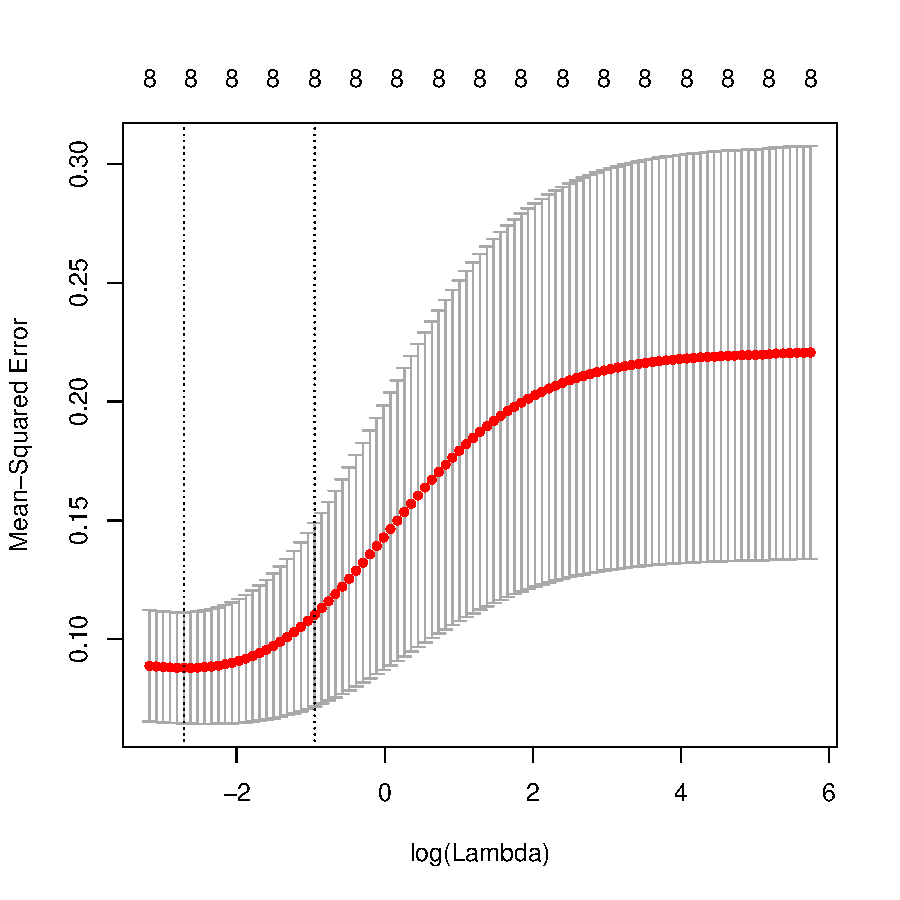
\includegraphics{crossvalidation-99c}

\part{d}
\begin{Schunk}
\begin{Sinput}
> ridge.mod = glmnet(x.train, y.train, alpha = 1, lambda = grid, thresh = 1e-12)
> cv.out = cv.glmnet(x.train, y.train, alpha = 1)
> plot(cv.out)
> bestlam = cv.out$lambda.min
> bestlam
\end{Sinput}
\begin{Soutput}
[1] 0.008357777
\end{Soutput}
\begin{Sinput}
> ridge.pred = predict(ridge.mod, s = bestlam, newx = x.test)
> lasso.mrs = mean((ridge.pred - y.test) ^ 2)
> lasso.mrs
\end{Sinput}
\begin{Soutput}
[1] 0.05464687
\end{Soutput}
\begin{Sinput}
> lasso.coef = predict(cv.out, type = 'coeff', s = bestlam)
> lasso.coef
\end{Sinput}
\begin{Soutput}
9 x 1 sparse Matrix of class "dgCMatrix"
                       1
(Intercept)  4.370137313
blood        0.050607955
prog         0.009716315
enz          0.011266202
liver        0.116956233
age         -0.002251710
female       0.024308981
modAlc       .          
heavyAlc     0.391001280
\end{Soutput}
\end{Schunk}
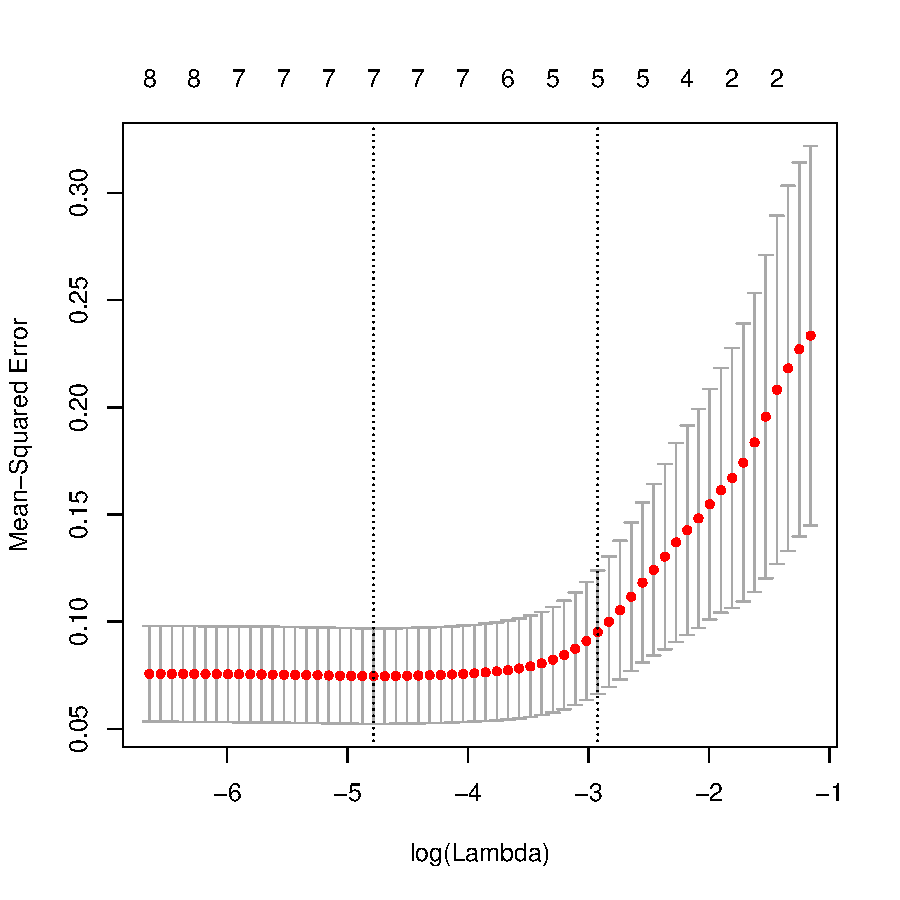
\includegraphics{crossvalidation-99d}

\part{g}
{\color{red}
\begin{enumerate}
\item We get a test error of 0.053 for linear model; 0.064 for ridge; 0.054 for lasso
\item The test error get from ridge and lasso are higher than test error directly from a linear mode.
\item From lass we see that coeff of predictor modAlc is set zero.
\end{enumerate}
}

\begin{Schunk}
\begin{Sinput}
> y.test.mu = mean(y.test)
> lm.r2 = 1 - mrs / mean((y.test - y.test.mu) ^ 2)
> ridge.r2 = 1 - ridge.mrs /mean((y.test - y.test.mu) ^ 2)
> lasso.r2 = 1 - lasso.mrs / mean((y.test - y.test.mu) ^ 2)
> lm.r2
\end{Sinput}
\begin{Soutput}
[1] 0.7983984
\end{Soutput}
\begin{Sinput}
> ridge.r2
\end{Sinput}
\begin{Soutput}
[1] 0.7581698
\end{Soutput}
\begin{Sinput}
> lasso.r2
\end{Sinput}
\begin{Soutput}
[1] 0.7921144
\end{Soutput}
\end{Schunk}
{\color{red}
\begin{enumerate}
\item From the $R^2$ statistic we can see that these three model only explained 79\% of the variance of the data, so the accuracy of our model is moderate.
\end{enumerate}
}
\end{document}
